\chapter{Sound, Oscillators, and the Deferred Second Law}

These companion notes follow Leonard Susskind's seventh lecture on statistical mechanics, with the present draft assembled from the lecture transcript and selected board frames curated by LazyingArt LLC and Video2Book. The lecture announces the second law immediately, but then deliberately postpones it. Before we tackle irreversibility, we first ask what statistical mechanics can already compute for us in concrete systems: the speed of sound in a dilute gas, the thermal energy of a harmonic oscillator, and the way quantum mechanics freezes or activates degrees of freedom. Only after that long preparation do we come back to the real conceptual puzzle.

\section{Why We Delay the Second Law}

The lecture opens with a promise: eventually we are going to discuss the second law, what it means, and how it can possibly be consistent with reversible microscopic laws. But it is a good promise to delay. If we start with entropy too soon, the subject can sound like a slogan. If instead we begin with examples that already show the power of statistical mechanics, then when the second law appears it comes attached to working mathematics.

That is the order we will preserve. We first look at a dilute gas and ask for the speed with which an overdensity spreads. Then we turn to the harmonic oscillator in a heat bath and discover an answer which is mathematically correct classically and yet physically crazy. That paradox is what invites quantum mechanics in. Only after that do we return to the second law itself.

\section{Speed of Sound in a Dilute Gas}

Susskind begins with a very physical question. Suppose we make a slightly overdense region in a very dilute gas. How fast does that excess density spread? In a gas dilute enough that molecules essentially carry information by moving, one naturally guesses that the relevant speed should be comparable to the molecular speed itself.

So we first estimate the molecular speed from equipartition. In thermal equilibrium each molecule carries kinetic energy
\begin{equation}
\frac{3}{2}k_B T=\frac{1}{2}m\langle v^2\rangle.
\end{equation}
Therefore
\begin{equation}
\langle v^2\rangle=\frac{3k_B T}{m}.
\end{equation}
At this stage the point is not precision. The point is that in a dilute gas the speed of sound should be of the same order as the molecular speed, because the overdensity spreads by molecules moving out of the dense region.

He then pivots to the more formal formula. At lecture level, and without pausing over the full hydrodynamic derivation, we write
\begin{equation}
v_s^2=\frac{\partial P}{\partial \rho_{\mathrm{mass}}}.
\end{equation}
If \(\rho\) denotes the particle number density and \(\rho_{\mathrm{mass}}=m\rho\) the mass density, then this becomes
\begin{equation}
v_s^2=\frac{1}{m}\frac{\partial P}{\partial \rho}.
\end{equation}
For an ideal gas,
\begin{equation}
PV=Nk_B T,
\qquad
P=\rho k_B T.
\end{equation}
Differentiating with respect to \(\rho\) at fixed temperature gives
\begin{equation}
\frac{\partial P}{\partial \rho}=k_B T,
\end{equation}
and therefore
\begin{equation}
v_s^2=\frac{k_B T}{m}.
\end{equation}

This does not exactly reproduce the naive molecular-speed estimate. The heuristic argument gave \(3k_B T/m\) for the typical molecular \(v^2\), while the more formal sound-speed formula gives \(k_B T/m\). So the crude estimate is off by a factor of \(3\) in \(v^2\), or \(\sqrt{3}\) in \(v\). In the lecture that discrepancy is not swept away. It remains part of the point: the first estimate is an order-of-magnitude argument, not a finished theory.

The numerical estimate for air is still revealing. Taking
\begin{equation}
k_B \approx 1.3\times 10^{-23}\,\mathrm{J/K},
\qquad
T\approx 300\,\mathrm{K},
\qquad
m_{\mathrm{air}}\approx 4\times 10^{-26}\,\mathrm{kg},
\end{equation}
one gets a speed of a few hundred meters per second. Using the naive estimate gives about \(500\,\mathrm{m/s}\); dividing by \(\sqrt{3}\) brings it down to roughly \(300\,\mathrm{m/s}\), which is the right scale.

The student interruptions matter here. One asks whether the factor of \(3\) should disappear because sound propagates in one direction. Susskind does not pretend to settle that cleanly on the spot; he leaves it as a serious question but insists that the order of magnitude is right. Another asks about the assumption that temperature is held fixed. Again the answer is lecture-level and cautious: for small-amplitude sound waves in a nearly ideal gas, treating the temperature variation as negligible is probably a good approximation. Yet another asks whether the speed of sound should depend on pressure. The response is that it does through the equation of state: outside the ideal-gas regime, \(\partial P/\partial \rho\) need not remain constant.

So the gas example does exactly the work it is supposed to do. It shows how statistical mechanics gives us a concrete scale, and it reminds us at the same time that we are often reasoning with approximations whose domain has to be watched carefully.

\section{A Classical Harmonic Oscillator in a Heat Bath}

Now we move on. Instead of a free particle in a gas, we place a single harmonic oscillator in a heat bath and ask for its average energy. This is the real mathematical center of the first half of the lecture.

A one-dimensional harmonic oscillator has Hamiltonian
\begin{equation}
H(x,p)=\frac{p^2}{2m}+\frac{\kappa x^2}{2}.
\end{equation}
Here \(x\) is the displacement from equilibrium, \(p\) is the momentum, and \(\kappa\) is the spring constant. From this point on, as in the lecture, we suppress \(k_B\), so that \(\beta=1/T\).

The Boltzmann weight is
\begin{equation}
e^{-\beta H}=e^{-\beta p^2/2m}\,e^{-\beta \kappa x^2/2}.
\end{equation}
The partition function is therefore
\begin{align}
Z_{\mathrm{cl}}
&=\int dp\,dx\,e^{-\beta H(x,p)} \\
&=\left(\int dp\,e^{-\beta p^2/2m}\right)
  \left(\int dx\,e^{-\beta \kappa x^2/2}\right).
\end{align}
So the whole problem reduces to two Gaussian integrals.

For the momentum integral we define
\begin{equation}
q^2=\frac{\beta p^2}{2m},
\qquad
dp=\sqrt{\frac{2m}{\beta}}\,dq.
\end{equation}
For the position integral we similarly define
\begin{equation}
y^2=\frac{\beta \kappa x^2}{2},
\qquad
dx=\sqrt{\frac{2}{\beta\kappa}}\,dy.
\end{equation}
Each integral then becomes a numerical constant times a factor of \(\beta^{-1/2}\). The numerical constants do not matter for the average energy, because they only add constants to \(\log Z\). Multiplying the two pieces together gives
\begin{equation}
Z_{\mathrm{cl}}=\frac{2\pi}{\omega}\frac{1}{\beta},
\qquad
\omega=\sqrt{\frac{\kappa}{m}},
\end{equation}
up to the same kind of irrelevant multiplicative constant that never survives differentiation of \(\log Z\).

\begin{figure}[h]
\centering

\includegraphics[width=0.47\textwidth]{lecture_07_figure_02.png}\hfill

\includegraphics[width=0.47\textwidth]{lecture_07_figure_03.png}
\caption{The end of the classical oscillator calculation on the board. The right frame gives the clearest evidence for the final identification \(E=1/\beta=T\), while the upper \(\log Z\) line remains partly occluded in both frames.}
\end{figure}

The board is partially blocked at exactly the point where the algebra is about to become conceptual. The cautious reconstruction consistent with the visible lines and with the derivation is
\begin{align}
\log Z_{\mathrm{cl}}&=\text{const}-\log\beta,\\
E&=-\frac{\partial \log Z_{\mathrm{cl}}}{\partial \beta}
=\frac{1}{\beta}
=T.
\end{align}

This is the result the lecture wants us to feel, not merely record. A one-dimensional classical oscillator in a heat bath has average energy \(T\).

At first glance one might compare this with the \(3T/2\) for a gas particle and ask: where did the \(3\) go, and where did the \(1/2\) go? The answer is pedagogically important. There is no factor of \(3\) because we are now looking at a one-dimensional oscillator, not a particle moving in three translational directions. And there is no overall \(1/2\) because there are two Gaussian integrals, one from momentum and one from position. Each quadratic contribution gives half a temperature:
\begin{equation}
\langle K\rangle=\frac{T}{2},
\qquad
\langle U\rangle=\frac{T}{2},
\qquad
\langle H\rangle=T.
\end{equation}
Thus the kinetic and potential parts are equal on average, and together they produce the full temperature.

Two features of the answer are already striking. It does not depend on the mass \(m\). And it does not depend on the spring constant \(\kappa\). The mass-independence resembles what we already saw for free particles in a gas: the velocities change with \(m\), but the mean kinetic energy does not. The \(\kappa\)-independence is the more surprising part, and it is the hinge on which the next transition turns.

\subsection{Question \& Answer}

\paragraph{Question.} Why does an infinitely stiff oscillator not stay frozen? If \(\kappa\) becomes enormous, should not the oscillator become impossible to excite?

\paragraph{Answer.} Classically, the algebra simply does not care. The spring constant appears in the partition function only inside an overall multiplicative factor,
\begin{equation}
Z_{\mathrm{cl}}\propto \sqrt{\frac{m}{\kappa}}\frac{1}{\beta}.
\end{equation}
Once we take the logarithm, that \(\kappa\)-dependence becomes an additive constant. Differentiating with respect to \(\beta\) removes it, and the average energy remains \(E=T\). So the conclusion is not a slip of the calculation. It is a correct classical conclusion.

That is exactly the problem. If the spring is so stiff that no reasonable force can displace it, common sense says it should carry essentially no internal energy. Yet classical statistical mechanics assigns \(T\) to it anyway. The lesson is not that the classical derivation was done badly. The lesson is that we have omitted a crucial feature of nature. The missing ingredient is quantum mechanics.

\section{Quantum Oscillator and Activated Degrees of Freedom}

Susskind now brings in the minimum quantum input needed to resolve the paradox. We do not need Hilbert space technology. We only need the quantized energy levels of the harmonic oscillator. In the lecture convention, before a later student question restores the zero-point term, the levels are taken to be
\begin{equation}
E_n=n\hbar\omega,
\qquad n=0,1,2,\dots
\end{equation}
The quantum partition function is therefore
\begin{equation}
Z_{\mathrm{q}}=\sum_{n=0}^{\infty}e^{-\beta n\hbar\omega}.
\end{equation}
This is just a geometric series:
\begin{equation}
Z_{\mathrm{q}}
=\sum_{n=0}^{\infty}\left(e^{-\beta\hbar\omega}\right)^n
=\frac{1}{1-e^{-\beta\hbar\omega}}.
\end{equation}

We now compute the mean energy. Using the standard relation,
\begin{equation}
E=-\frac{\partial \log Z_{\mathrm{q}}}{\partial \beta},
\end{equation}
or equivalently \(E=-(1/Z_{\mathrm{q}})\,\partial Z_{\mathrm{q}}/\partial\beta\), we obtain
\begin{equation}
E=\hbar\omega\,\frac{e^{-\beta\hbar\omega}}{1-e^{-\beta\hbar\omega}}.
\end{equation}
If one wants the more familiar cleaned form, this is
\begin{equation}
E=\frac{\hbar\omega}{e^{\beta\hbar\omega}-1},
\end{equation}
but the lecture keeps the unsimplified version in view because it makes the limiting regimes easier to read.

At high temperature, \(\beta\hbar\omega\ll 1\). Expanding the exponential in the denominator gives
\begin{equation}
1-e^{-\beta\hbar\omega}\approx \beta\hbar\omega,
\end{equation}
and therefore
\begin{equation}
E\approx \frac{\hbar\omega}{\beta\hbar\omega}=\frac{1}{\beta}=T.
\end{equation}
So the quantum oscillator reproduces the classical answer in the high-temperature limit. This is the right logic of the subject: quantum mechanics first, classical statistical mechanics as a limit case.

At low temperature, \(\beta\hbar\omega\gg 1\), so the exponential is tiny. Then
\begin{equation}
E\approx \hbar\omega\,e^{-\beta\hbar\omega},
\end{equation}
which is exponentially small in the lecture's shifted-energy convention. Thus quantum mechanics suppresses the excitation of the oscillator when the temperature is too low.

The crossover occurs when the exponential ceases to be clearly close to \(1\) or clearly tiny, namely when
\begin{equation}
\beta\hbar\omega\sim 1
\qquad\Longleftrightarrow\qquad
T\sim \hbar\omega.
\end{equation}
This is the threshold equation the lecture wants us to interpret physically. The classical oscillator carries energy \(T\). A quantum oscillator can only absorb energy in lumps of size \(\hbar\omega\). So the classical description becomes valid precisely when the thermal energy reaches the size of one quantum.

This resolves the stiff-spring paradox. A stiffer oscillator has larger frequency,
\begin{equation}
\omega=\sqrt{\frac{\kappa}{m}},
\end{equation}
so its threshold temperature is higher. Above that threshold it behaves classically and carries energy \(T\). Below that threshold it is effectively frozen out.

There is a nice practical clarification in the lecture. If we heat an oscillator above the threshold, the spring does not somehow become tighter. What changes is the motion: larger oscillation amplitude, higher momentum, larger energy. The independence of \(E=T\) from \(\kappa\) is not a statement about all temperatures. It is a statement about the classical regime, and the temperature at which that regime begins climbs upward as the spring becomes stiffer.

\paragraph{Activated degrees of freedom.} Once this threshold picture is in place, Susskind broadens it immediately. A diatomic molecule has vibrational structure, but if the vibrational quantum is too large compared with the temperature, the molecule behaves thermally as if that vibration were absent. At low temperature it looks effectively monatomic. Raise the temperature past the threshold, and the vibrational degree of freedom switches on. Raise it further, and additional structures appear: rotational motion, internal vibrations of constituents, eventually ionization.

The same logic applies to solids. A crystal is a collection of oscillators. Classically one would assign too much energy, and therefore too large a specific heat, to those oscillators. Einstein's early insight was that quantum mechanics suppresses the modes until the temperature becomes large enough to activate them.

For many independent oscillators we have
\begin{equation}
Z_{\mathrm{tot}}=\prod_i Z_i,
\qquad
\log Z_{\mathrm{tot}}=\sum_i \log Z_i,
\qquad
E_{\mathrm{tot}}=\sum_i E_i.
\end{equation}
So the total energy is just the sum of the mode energies. But the important point is that not all modes contribute equally. If
\begin{equation}
\hbar\omega_i\gg T,
\end{equation}
then the \(i\)-th mode is deep in the quantum regime and its contribution is exponentially suppressed.

That is why the violin-string image works so well. Mathematically, a vibrating string is a superposition of infinitely many harmonic oscillators, one for each normal mode. If each mode carried energy \(T\), the string would have infinite thermal energy. Quantum mechanics prevents that catastrophe. High-frequency, short-wavelength modes have \(\hbar\omega\) far above the temperature and are frozen out. As the temperature rises, more and more modes become active.

\paragraph{A later question: the zero-point energy.} Near the end of this discussion a student asks about the missing \(\frac12\hbar\omega\). The physical spectrum is
\begin{equation}
E_n^{\mathrm{phys}}=\left(n+\frac12\right)\hbar\omega.
\end{equation}
Why was it harmless to omit the extra \(\frac12\hbar\omega\)? Because adding the same constant to every energy level multiplies the partition function by the same factor:
\begin{equation}
Z_{\mathrm{phys}}=e^{-\beta\hbar\omega/2}Z_{\mathrm{q}}.
\end{equation}
That only adds a constant to \(\log Z\), and the temperature-dependent conclusions obtained from differentiating \(\log Z\) are unchanged.

\section{Back to the Second Law: Phase Space, Liouville, and Coarse-Graining}

Only now does the lecture return to its announced destination. Why is the second law a puzzle? Because the second law says that entropy increases, or at least does not decrease, while the microscopic equations of motion are reversible. Anything that can happen forward can happen backward. So where does irreversibility come from?

The first move is geometric. We imagine phase space, the space of all states of a classical system. For a many-particle system it is enormously high-dimensional, but we draw it schematically as a plane with one axis representing positions and the other momenta. Suppose that our knowledge of the system is limited to the statement that its phase point lies somewhere inside a certain patch. The probability density is uniform inside that patch and zero outside.

For such a uniform distribution it is natural to associate the entropy with the size of the occupied region:
\begin{equation}
S_{\mathrm{micro}}\propto \log V_{\mathrm{blob}}.
\end{equation}
In the lecture there is a brief verbal wobble about a minus sign, but the reasoning that follows is clear: larger occupied volume means less information and therefore larger entropy.

Now evolve the system in time. Liouville's theorem says that Hamiltonian flow preserves phase-space volume:
\begin{equation}
V_{\mathrm{blob}}(t)=V_{\mathrm{blob}}(0).
\end{equation}
So if we follow the exact fine-grained patch with infinite precision, the occupied region may bend and stretch, but its volume remains unchanged. At that level the entropy does not increase.

\begin{figure}[h]
\centering
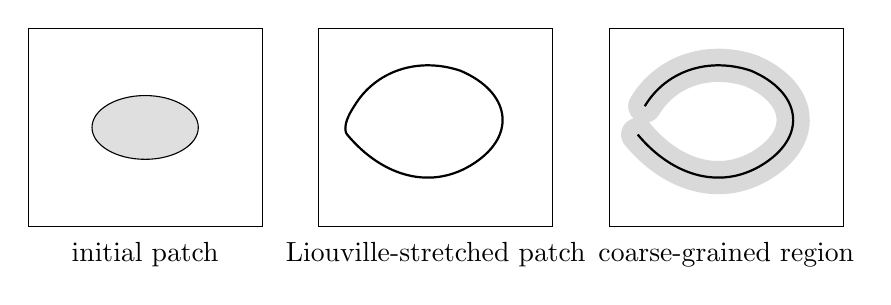
\begin{tikzpicture}[scale=0.9]
\draw (-0.5,-1.4) rectangle (2.8,1.4);
\fill[gray!25] (1.15,0) ellipse (0.75 and 0.45);
\draw (1.15,0) ellipse (0.75 and 0.45);
\node at (1.15,-1.8) {initial patch};

\draw (3.6,-1.4) rectangle (6.9,1.4);
\draw[line width=0.8pt]
(4.0,-0.1) .. controls (4.5,-0.7) and (5.2,-0.9) .. (5.8,-0.5)
.. controls (6.4,-0.1) and (6.3,0.5) .. (5.6,0.8)
.. controls (5.0,1.0) and (4.4,0.8) .. (4.1,0.3)
.. controls (3.9,0.0) and (4.0,-0.1) .. (4.0,-0.1);
\node at (5.25,-1.8) {Liouville-stretched patch};

\draw (7.7,-1.4) rectangle (11.0,1.4);
\draw[line width=12pt, gray!30, line cap=round]
(8.1,-0.1) .. controls (8.6,-0.7) and (9.3,-0.9) .. (9.9,-0.5)
.. controls (10.5,-0.1) and (10.4,0.5) .. (9.7,0.8)
.. controls (9.1,1.0) and (8.5,0.8) .. (8.2,0.3);
\draw[line width=0.8pt]
(8.1,-0.1) .. controls (8.6,-0.7) and (9.3,-0.9) .. (9.9,-0.5)
.. controls (10.5,-0.1) and (10.4,0.5) .. (9.7,0.8)
.. controls (9.1,1.0) and (8.5,0.8) .. (8.2,0.3);
\node at (9.35,-1.8) {coarse-grained region};
\end{tikzpicture}
\caption{The lecture's geometric logic: an initially compact patch flows into a thin filamentary ``snake'' of the same volume, while coarse-graining replaces that fine structure by a larger effective occupied region.}
\end{figure}

\subsection{Question \& Answer}

\paragraph{Question.} If Liouville's theorem preserves phase-space volume exactly, how can entropy possibly increase?

\paragraph{Answer.} It cannot increase at the fully resolved microscopic level. The key point is that the entropy relevant to the second law is not the entropy of a perfectly known fine-grained distribution. It is an entropy defined relative to what we can actually distinguish. Real measurements do not resolve arbitrarily thin filamentary structure. So a patch that has been stretched into a long thin snake is no longer represented as a thin snake; it is replaced by finite-resolution blobs. Those blobs cover a region larger than the original patch, and therefore the coarse-grained entropy increases.

In other words, entropy is not just a property of the system by itself. It is a property of the system together with the level of information we retain about it. If we track every microscopic detail, entropy stays constant. If we describe the system at finite resolution, entropy grows.

This is the cotton analogy in the lecture. The fibers themselves may occupy only a small total volume, but once the cotton is allowed to fluff out, a coarse observer sees a much larger object. Likewise a phase-space patch keeps its exact Liouville volume while its coarse-grained extent increases.

What makes this robust is chaos. A phase-space patch does not merely stretch once. It develops thinner and thinner tendrils, and those develop finer tendrils still. No matter how good the resolution is, wait long enough and the dynamics will produce structure below that resolution.

That is the real role of chaos in the lecture. A chaotic system is one in which nearby trajectories stay close for a while and then separate, so predictability breaks down unless one knows the initial state with increasing precision. The harmonic oscillator is the counterexample: nearby phase points circle together forever. A true two-body Kepler problem is likewise non-chaotic. A three-body problem is generically chaotic. The double pendulum is chaotic. The billiard-table analogy is used for the same reason: not because the balls fill the table itself, but because the trajectory explores the space of possibilities.

\begin{figure}[h]
\centering
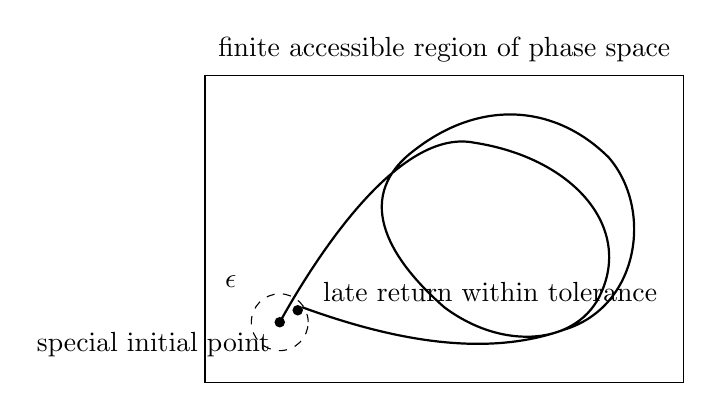
\begin{tikzpicture}[scale=0.95]
\draw (0,0) rectangle (6.4,4.1);
\node at (3.2,4.45) {finite accessible region of phase space};

\fill (1.0,0.8) circle (2pt);
\node[below left] at (1.0,0.8) {special initial point};

\draw[dashed] (1.0,0.8) circle (0.38);
\node[left] at (0.55,1.35) {\(\epsilon\)};

\draw[line width=0.8pt]
(1.0,0.8) .. controls (1.5,1.7) and (2.6,3.4) .. (3.6,3.2)
.. controls (4.9,3.0) and (5.7,2.1) .. (5.3,1.2)
.. controls (5.0,0.5) and (4.0,0.4) .. (3.2,1.0)
.. controls (2.4,1.7) and (2.0,2.5) .. (2.8,3.1)
.. controls (3.7,3.8) and (4.7,3.7) .. (5.4,3.0)
.. controls (6.0,2.3) and (5.8,1.0) .. (4.8,0.7)
.. controls (3.7,0.3) and (2.4,0.6) .. (1.3,1.0);

\fill (1.24,0.96) circle (2pt);
\node[right] at (1.45,1.2) {late return within tolerance};

\end{tikzpicture}
\caption{A schematic recurrence picture. The exact phase point wanders through a bounded accessible region and, after a typically enormous time, can return to an \(\epsilon\)-neighborhood of its starting point.}
\end{figure}

The lecture then adds an essential refinement. Coarse-grained entropy increase does not mean exact non-return. If the accessible phase-space region is finite, then over a long enough time the system can come arbitrarily close to where it started. But the statement has to be made with tolerance. We do not require exact return to the original point; we require return to an \(\epsilon\)-neighborhood of it. For any fixed tolerance, the return time is finite, though usually unimaginably large.

This is where reversibility re-enters. The same system whose coarse-grained entropy grows can, in principle, return near its initial special configuration. So the second law is not a theorem that entropy literally always increases without exception. Boltzmann's resolution is probabilistic: from a given configuration, the next one is overwhelmingly more likely to have larger entropy than smaller entropy. Entropy probably increases.

That is a weaker sentence than the slogan, but it is the right one. It is also stronger physically, because it is the form that actually fits the reversible microscopic laws together with the enormous imbalance of probabilities in many-body systems.

\section{Summary}

The lecture's path is deliberate. We begin with a dilute gas and learn that statistical mechanics can already give us the right scale for the speed of sound. We then turn to the classical harmonic oscillator and find the beautiful but disturbing result \(E=T\), with \(T/2\) in kinetic and \(T/2\) in potential energy. That result becomes absurd for very stiff oscillators, and quantum mechanics repairs it by introducing the threshold \(T\sim\hbar\omega\). Once that threshold is understood, whole families of physical phenomena fall into place: molecular vibrations, crystal specific heat, and the freezing-out of high-frequency modes.

Only then do we return to the second law. Exact Hamiltonian evolution preserves phase-space volume, but coarse-grained descriptions do not preserve the effective occupied volume of a filamented patch. That is how entropy can increase without contradicting reversibility. The price of the resolution is that the second law becomes probabilistic rather than absolute. For real systems, that is not a defect. It is the content.